\documentclass[italian,12pt,a4paper]{article}
\usepackage[utf8]{inputenc}
\usepackage[T1]{fontenc}
\usepackage{mathtools}
\usepackage{amsmath}
\usepackage{blkarray, bigstrut} %
\usepackage{babel}
\usepackage{graphicx}
\usepackage{subfig}
\usepackage{hyperref}
\usepackage{tikz}
\usepackage{colortbl}
\usepackage{pgf-pie}
\usepackage{algorithm}
\usepackage{algpseudocode}
\usepackage{algorithmicx}
\usepackage{placeins}
\usepackage{svg}
\usepackage{tabularx}
\title{Università degli studi di Bari facoltà di Informatica}
\date{} % clear date
\hypersetup{
	colorlinks=true,
	linkcolor=black,
	filecolor=magenta,      
	urlcolor=cyan,
	pdfpagemode=FullScreen,
}
\graphicspath{ {./img/} }
\RequirePackage[subfigure]{tocloft}

\cftsetindents{section}{0em}{2em}
\cftsetindents{subsection}{0em}{2em}

\renewcommand\cfttoctitlefont{\hfill\Large\bfseries}
\renewcommand\cftaftertoctitle{\hfill\mbox{}}

\algrenewcommand\algorithmicrequire{\textbf{Input:}}
\algrenewcommand\algorithmicensure{\textbf{Output:}}

\setcounter{tocdepth}{2}
\begin{document}
	\maketitle
	\thispagestyle{empty}
	\begin{center}
		\huge	\textbf{Progetto di Data Mining} \\
		\Large \textbf{HCV DM23 Liver fibrosis staging classification}
	\end{center}
	
	
	
	\begin{center}
		a cura di \\
		\Large \textbf{Diego Miccoli}
	\end{center}

	
	\begin{figure}[hb]
		\centering
		
\includegraphics[width=10cm]{logoUNIlatex.png}
	\end{figure}
	
	\vfill
	\begin{center}
		Anno accadenico 2022-2023
	\end{center}
	
	\newpage
	
	\tableofcontents

	\newpage

	
	\section{Introduzione}

	\subsection{HCV e problema affrontato}

	% \href{https://www.kaggle.com/datasets/sameepvani/nasa-nearest-earth-objects/}{Near-Earth Objects} (NEO)
    Lo sviluppo di questo progetto si basa sullo studio di un gruppo di medici Egiziani i quali hanno condotto delle indagini di ricerca sui danni provocati dal virus dell'epatite C sul fegato. Questo studio di ricerca è stato mosso dalla grave situazione di epidemiologia in cui si trova attualmente la nazione Egitto. Essa infatti assieme a Bolivia, Camerun, Guinea e Mongolia detendono il primato per maggior numero di contagi annui e per proliferazione del HCV nella popolazione. Questi paesi rappresentano i principali focolai maggiormente attivi nel mondo tuttavia HCV infetta ogni anno parecchi individui in Brasile nell'Africa centrale, est Europa e Asia, mentre nel resto del mondo grazie ad una adeguata prevenzione la diffusione è tenuta sotto controllo a livelli non allarmanti dal punto di vista della sanità. Questo team di medici Egiziani ha cercato di investigare sul epidemiologia del HCV in Egitto e su come questo si evolva all'interno dell'organismo umano e come porta all'insorgenza di fibrosi epatica che tenda a cronicizzare nel tempo.
    \\
	
	\subsection{Dati raccolti dallo studio dei medici sul HCV}
	I medici hanno raccolto un intero dataset che sarà quello che utilizzeremo per il progetto di data mining, il quale contiene dati biometrici dei pazienti presi in esame per lo studio sul HCV, i loro test ematici svolti per monitorare alcuni parametri e indicatori presenti nel sangue, i test delle transaminasi con particolare riguardo all'ALT ovvero alanina ammino trasferrasi, i test riguardanti l'attività di sintesi polimerica del HCV ovvero il processo con il quale il virus una volta che infetta le cellule del corpo umano, inizia una fase trascrittiva del proprio RNA per usare la cellula ospite come fabbrica per la replicazione e la diffusione. A corredo di questi dati infine vi sono generalità del paziente e due scale di valutazione del danno epatico. La prima scala è conosciuta in medicina con il nome di scala METAVIR ed essa prevede 4 livelli o stadi di fibrosi epatica, la seconda scala invece è un scala di uso recente ed attualmente non è utilizzata a livello globale in sanità o in medicina, questo perchè è stato il team dei medici sopra citato a idearla per avere un idea del danno epatico rispetto alla compromissione della funzionalità. La differenza tra le due scale sta nel fatto che la METAVIR identifica e classifica il danno epatico in base alla trasformazione degli epatociti in tessuto fibrotico ovvero tessuto che non ricopre le funzionalità del fegato, mentre la seconda cerca di quantificare la progeressione della fibrosi e quindi del problema epatico in base alla ridotta funzionalità del fegato e assume una scala di valori da 0 a 20.

	
	\subsection{La fibrosi epatica}
 
    La fibrosi epatica è una condizione in cui il tessuto cicatriziale si accumula nel fegato in risposta a danni cronici o ripetuti. Questa cicatrizzazione può verificarsi a causa di diverse cause, come l'epatite virale, l'uso cronico di alcol, le malattie autoimmuni del fegato, l'accumulo di grasso nel fegato (steatosi epatica non alcolica) o altre condizioni che causano danni al fegato nel tempo.
    La fibrosi epatica progredisce attraverso diversi stadi, noti come stadi di fibrosi o gradi di fibrosi. Esistono diversi sistemi di classificazione per valutare la fibrosi epatica, ma uno dei più comuni è il sistema METAVIR, che assegna un punteggio da F0 a F4 per descrivere l'estensione della fibrosi epatica. Ecco una breve descrizione di ciascun stadio secondo il sistema METAVIR:
    \\
    
    \begin{enumerate}
		\item \textbf{F0: Nessuna fibrosi },  Il fegato non mostra segni di cicatrizzazione o fibrosi significativa. Questo è considerato uno stadio normale senza cicatrizzazione.
		\item \textbf{F1: Fibrosi portale }, Si osserva una leggera fibrosi nella zona del portale, che è l'area intorno ai vasi sanguigni e ai dotti biliari nel fegato. La fibrosi è ancora relativamente limitata.
		\item \textbf{F2: Fibrosi portale con ponti }, La fibrosi è più marcata e si osservano ponti fibrosi tra le zone del portale adiacenti.
		\item \textbf{F3: Fibrosi settale}, La fibrosi si estende oltre le zone del portale e coinvolge le pareti dei setti, che sono le strutture interne del fegato che separano le unità funzionali chiamate lobi epatici. La cicatrizzazione è significativa, ma non ha ancora compromesso la struttura del fegato in modo critico.
		\item \textbf{F4: Cirrosi}, Questo è lo stadio più avanzato della fibrosi epatica in cui la cicatrizzazione del fegato è estensiva e irreversibile. La struttura del fegato è compromessa, con formazione di noduli cicatriziali che possono interferire con il normale flusso di sangue attraverso il fegato.
	\end{enumerate} 

    \vspace{25pt}
    
	È importante notare che la fibrosi epatica è un processo progressivo e che la presenza di fibrosi avanzata (stadio F3 o F4) indica un rischio elevato di sviluppare complicanze epatiche gravi, come l'insufficienza epatica o il carcinoma epatocellulare. Pertanto, è cruciale identificare e trattare la fibrosi epatica nelle fasi iniziali per prevenire la progressione a stadi più avanzati e proteggere la funzione epatica.

    \subsection{trattamento generale della fibrosi epatica e antivirale usato nello studio}
	I trattamenti generali per la fibrosi epatica legata alle infezioni da HCV includono l'uso di farmaci antivirali ad azione diretta DAA e misure per il sostegno del fegato volte a favorire la ripresa delle sue normali attività enzimatiche. Nello studio citato è stato scelto un trattamento con un antivirali chiamato Sobusbovir, in particolare questo farmaco agisce andando ad inibire l'attività polimerasi del virus andando quindi ad impedirne la replicazione all'interno della cellula. Durante il trattamento le attività di monitoraggio e follow-up regolari sono un must che risulta di vitale importanza per monitorare attentamente la risposta del paziente e l'evoluzione della fibrosi epatica. Ciò può comportare l'esecuzione di test di funzionalità epatica, test di carica virale e biopsie epatiche per valutare l'estensione della fibrosi e il grado di danno al fegato, ed infine ecografie addominali atte a valutare le dimensioni del fegato e l'accumulo di liquidi dovuti a mal funzionamento della vena portale. Modifiche dello stile di vita sono richieste durante e dopo il trattamento per supportare la salute del fegato e queste possono include l'astensione dal consumo di alcol e l'adozione di una dieta equilibrata ed evitare cibi ad alto contenuto di grassi. Risultano infine essenziali le informazioni di comprensione dello stato di salute del paziente e di un piano terapeutico volto a gestire la presenza di coomorbilità e altre patologie e l'uso di altri farmaci quest'ultimo punto è di vitale importanza in quanto il fegato è l'organo deputato allo smaltimento dei rifiuti del nostro organismo e allo smaltimento di sostanze quali i medicinali per tali ragione è essensiale una comprensione di questa sitauzione da parte del paziente.
    \\

	\subsection{Come la data mining può intervenire su questo problema}
    Alla luce di quanto detto fino ad ora ci chiediamo cosa possa centrare la data mining in tutto questo che sembra di dominio della medicina. Partiamo con il dire che ogni qualvolta che sono presenti dei dati in buone quantità la data mining è la risorsa che ci permette di estrarre tutte le pontenzialità intrinseche nei dati, ma non facilmente riconoscibili senza una attenta analisi. Questo processo porta quindi alla scoperta di nuove informazioni che si possono rilevare di vitale importanza, per tali ragioni il primo obiettivo che si pone questo progetto è quello di scoprire correlazioni utili tra i dati raccolti dai medici al fine di trarre conclusioni che permettano di agevolare la gestione e il trattamento di questi pazienti affetti da fibrosi epatica. Come secondo obiettivo il quale riveste il cardine della nostra ricerca e sperimentazione sarà quello di implementare dei modelli di machine learning supervisionati che permettano di utilizzare i dati raccolti per addestrare il modello in futuro a riconoscere a partire da tali dati, ovvero osservazioni laboratoristiche e esami diagnostici medici, la stadio attuale della fibrosi epatica di un dato paziente. Questo modello se riuscisse a realizzare tale predizione con buone performance di esattezza potrebbe integrare l'attività medico-sanitaria nelle procedure di diagnostica e trattamento di questi pazienti apportando notevoli risparmi in termine di esami diagnostici costosi che vengo ad essere evitati, quali ecografie e biopsie del tessuto epatico, con la conseguenza di alleggerire il carico di lavoro dei reparti ospedalieri adibiti al trattamento di questa patologia e la possibilità di donare una più serena convivenza con la malatia cronica al paziente che non dovrà sottoporsi ripetutamente a test dolorosi.
    \\
    
    \subsection{Cosa è e cosa studia la data mining}
    La data mining è il processo di scoperta di informazioni significative, modelli e relazioni all'interno di grandi quantità di dati. È una disciplina che combina concetti e tecniche provenienti da diverse aree, come l'intelligenza artificiale, la statistica , la matematica e l'analisi dei dati.
    L'obiettivo principale del data mining è estrarre conoscenze utili e previsioni da un insieme di dati, al fine di supportare la presa di decisioni informate. Attraverso l'applicazione di algoritmi sofisticati, il data mining analizza i dati alla ricerca di modelli nascosti, tendenze o anomalie che potrebbero non essere facilmente identificabili tramite metodi tradizionali. Per realizzare tutto quello che abbiamo appena descritto essa applica un processo analitico diviso in più fasi teso ad analizzare il problema sotto diversi aspetti e punti di vista con il fine di produrre un piano di azione e dei risultati da raggiungere. Esistono 2 principali metodologie per l'applicazione di tali processi che portano all'estrazione della conoscenza dai dati e questi sono:
    \\
    
    \begin{itemize}
			\item  \textbf{SEMMA}, sta per Sample, Explore, Modify, Model, e Assess ovvero le principali attività svolte. Questa metodologia fornisce una struttura organizzata per l'intero ciclo di vita del progetto di data mining.
			\item  \textbf{CRISP-DM}, Cross-Industry Standard Process for Data Mining è una metodologia ampiamente utilizzata per il processo di data mining che costa di 6 fasi. Permette  un approccio flessibile e iterativo che guida gli analisti attraverso le fasi chiave del progetto di data mining.   
		\end{itemize}

    \vspace{30pt}
    
   \section{Metodologie della data mining }
   
    \subsection{SEMMA}
    Il SAS Institute ha sviluppato SEMMA come processo di data mining. Si compone di cinque passaggi ( S ample, E xplore, M odify, M odel e A ssess), guadagnandosi l'acronimo di SEMMA. È possibile utilizzare la metodologia di data mining SEMMA per risolvere un'ampia gamma di problemi aziendali, tra cui l'identificazione delle frodi, la fidelizzazione e il turnover dei clienti, il database marketing, la fidelizzazione dei clienti, la previsione dei fallimenti, la segmentazione del mercato, nonché l'analisi del rischio, dell'affinità e del portafoglio. SEMMA è concepito come una metodologia di scienza dei dati per aiutare i professionisti a convertire i dati in conoscenza. Il processo SEMMA si scompone in una propria serie di fasi. Questi includono:

    \begin{enumerate}
		\item \textbf{Sample "Campione"}, In questa fase, viene selezionato un campione rappresentativo dai dati disponibili. Il campione è una porzione dei dati che verrà utilizzata per l'analisi e il modello di data mining. L'obiettivo di questa fase iniziale del processo è identificare variabili o fattori (sia dipendenti che indipendenti) che influenzano il processo. Le informazioni raccolte vengono quindi ordinate in categorie di preparazione e convalida.
		\item \textbf{Explore "Esplorare"}, vengono esplorati i dati per comprendere la loro struttura e distribuzione. Vengono utilizzati metodi statistici e visualizzazioni per individuare relazioni, tendenze, anomalie o pattern significativi. Attraverso l'analisi multivariata si studia la relazione tra le variabili, mentre con quella univariata si esamina ciascun fattore individualmente per comprendere la sua parte nello schema generale.
		\item \textbf{Modify "Modificare"}, lezioni apprese nella fase di esplorazione dai dati raccolti nella fase di campionamento vengono derivate con l'applicazione della logica aziendale. In altre parole, i dati vengono analizzati e puliti applicando trasformazioni o modifiche ai dati stessi per migliorarne la qualità, la coerenza o la rilevanza per l'analisi. Queste modifiche possono includere la pulizia dei dati, l'eliminazione di valori mancanti o outlier, la normalizzazione delle variabili.
		\item \textbf{Model "Modellizzare"}, vengono creati modelli statistici o algoritmi di data mining per estrarre conoscenze dai dati. Questi modelli possono includere tecniche come clustering, classificazione, regressione o associazione, a seconda degli obiettivi dell'analisi.
		\item \textbf{Assess "Valutare"}, i modelli creati vengono valutati e testati utilizzando dati aggiuntivi o attraverso tecniche di validazione incrociata. L'obiettivo è valutare l'accuratezza e l'affidabilità dei modelli e identificare eventuali miglioramenti o ottimizzazioni necessarie.
	\end{enumerate}

    \vspace{25pt}
    
    \subsection{KDD Knowledge discovery from data}
    Il termine derriva da knowledge discovery in databases indica l'intero processo di ricerca di nuova conoscenza dai dati. Nella data mining si riferisce all'applicazione di algoritmi per estrarre pattern dai dati. Quindi il KDD è un processo con il quale si affronta lo studio dei dati per estrarne conoscenza e si basa sui seguenti passi:

    \begin{enumerate}
		\item \textbf{Analisi del dominio applicativo}, Sviluppo e approfondimento del dominio di applicazione, della conoscenza disponibile a priori e degli obiettivi dell'utente finale.
		\item \textbf{Creazione di un target data set}, selezione del data set o focalizzazione su un sottoinsieme di variabili o di campioni di dati oggetto del processo KDD.
		\item \textbf{Cleaning dei dati e preprocessing:},  operazioni di base come la rimozione del rumore o degli outliers se è il caso, raccolta delle informazioni necessarie per modellare o tener conto del rumore, messa a punto di strategie per gestire i dati mancanti e per gestire i dati tempo-varianti.
		\item \textbf{Riduzione dei dati e proiezione}, rappresentazione dei dati in modo opportuno in relazione agli obiettivi della ricerca. Riduzione delle dimensioni e impiego di metodi di trasformazione per ridurre l'effettivo numero di variabili da sottoporre al processo di ricerca. 
		\item \textbf{Scelta del compito del processo di data mining}, identificazione dell'obiettivo del KDD, stabilire, cioè se si tratti di una classificazione, di una regressione, di un clustering.
		\item \textbf{Scelta dell'algoritmo o degli algoritmi di data mining}, selezione dei metodi da usare per ricercare pattern nei dati. Questa fase comprende la decisione su quali modelli e parametri potrebbero essere appropriati e il matching di un particolare metodo di data mining con i criteri generali del processo KDD.
        \item \textbf{Data mining}, ricerca di pattern di interesse in una particolare forma di rappresentazione o su un set di rappresentazioni diverse. Il risultato del processo di data mining è considerevolmente influenzato dalla correttezza delle fasi precedenti.
        \item \textbf{Interpretazione dei pattern trovati}, analisi dei risultati prodotti e della necessità di ritornare su step precedenti per corroborare i pattern trovati.
        \item \textbf{Consolidamento della conoscenza estratta}, incorporazione di tale conoscenza nel sistema di performance o, semplicemente, documentazione e reporting alle parti interessate. Questa fase include anche il controllo per la risoluzione di potenziali contraddizioni con la conoscenza precedentemente disponibile.
	\end{enumerate}

    \vspace{25pt}
    
    \subsection{Crisp-DM}
    Il  Cross  Industry Standard  Process for  Data  Mining meglio conosciuto come CRISP-DM  è un modello di processo che funge da base per un processo di  data science. Fu pubblicato per la prima volta nel 1999 con l'obiettivo di standardizzare i processi di data mining in tutti i settori industriali volti a scoprire nuova conoscenza dai dati e a prendere decisioni per le aziende in base all'analisi di tali dati. In particolare il CRISP-DM si compone di sei fasi:
	
	\begin{enumerate}
		\item \textbf{Buisness understanding}, dove si studia e si comprende il dominio applicativo e gli obiettivi da raggiungere, andando a produrre un project plan. Questa prima fase consta a sua volta di più sotto-fasi quali \textbf{Determina gli obiettivi di business} per comprendere a fondo, dal punto di vista del business, ciò che il cliente vuole veramente ottenere. \textbf{Valutare la situazione}  per determinare la disponibilità delle risorse, i requisiti del progetto, valutare i rischi e le contingenze e condurre un'analisi costi-benefici. \textbf{Determinare gli obiettivi di data mining} sewrve per definire gli obiettivi di business, è necessario anche definire l'aspetto del successo dal punto di vista del data mining tecnico. \textbf{Produzione del piano di progetto} seleziona tecnologie e strumenti e definisci piani dettagliati per ogni fase del progetto.
		\item \textbf{Data understanding}, fase nella quale si identificano metodi per l'acquisizione dei dati, problemi legati a quest'ultimi, come la qualità, gli errori, etc.., quì avviene la fase di esplorazione preliminare del dataset. Anche questa fase consta di 4 sotto-fasi \textbf{Raccolta  dati iniziali} acquisisci i dati necessari e (se necessario) caricali nel tuo strumento di analisi. \textbf{Descrivi i dati} esamina i dati e documenta le proprietà della superficie come il formato dei dati, il numero di record o le identità dei campi. \textbf{Esplora i dati} scava più a fondo nei dati. Interrogalo, visualizzalo e identifica le relazioni tra i dati. \textbf{Verifica la qualità dei dati} Quanto sono puliti/sporchi i dati? Documentare eventuali problemi di qualità.
		\item \textbf{Data preparation}, preparazione del dataset(s) andando a determinare il sottoinsieme dei dati che più rappresenta il dataset in funzione degli obiettivi, pulendo il dataset da errori, valori mancanti, \textit{outliers} ed attributi non funzionali allo scopo (feature selection), attuare tecniche per andare a ribilanciare i dati e così via. le sotto-fasi sono le seguenti Selezionare i dati: determinare quali set di dati verranno utilizzati e documentare i motivi dell'inclusione/esclusione. \textbf{pulitura dei dati} spesso questa è l'attività più lunga. Senza di esso, probabilmente cadrai vittima di immondizia in entrata e in uscita. Una pratica comune durante questa attività consiste nel correggere, imputare o rimuovere valori errati. \textbf{Costruizione dei dati} deriva nuovi attributi che saranno utili. Ad esempio, ricavare l'indice di massa corporea di qualcuno dai campi altezza e peso.\textbf{Integrazione dei dati} crea nuovi set di dati combinando i dati provenienti da più fonti. \textbf{Formattazione dei dati} riformatta i dati se necessario. Ad esempio, potresti convertire i valori stringa che memorizzano i numeri in valori numerici in modo da poter eseguire operazioni matematiche.
		\item \textbf{Modeling}, fase in cui si selezionano le tecniche di modeling andando a scegliere gli algoritmi da provare ed eseguendoli con i dovuti parametri, per poi andare a valutarli con le opportune metriche. le sotto-fasi sono le seguenti \textbf{Seleziona le tecniche di modellazione} determina quali algoritmi provare. \textbf{Genera progettazione di test} in attesa del tuo approccio di modellazione, potresti dover suddividere i dati in set di addestramento, test e convalida. \textbf{Modello di costruzione} addestramento del modello scelto. \textbf{Modello di valutazione} in genere, più modelli competono l'uno contro l'altro e il data scientist deve interpretare i risultati del modello in base alla conoscenza del dominio, ai criteri di successo predefiniti e alla progettazione del test.
		\item \textbf{Evaluation}, fase di confronto fra il data scientist ed il buisness owner per andare a valutare i risultati ottenuti in relazione agli obiettivi di buisness. Le sue sotto-fasi sono le seguenti \textbf{Valutare i risultati} per capire se i modelli soddisfano i criteri di successo aziendale. \textbf{Processo di revisione} rivedere il lavoro svolto. Controllare che tutti i passaggi sono stati eseguiti correttamente. Infine riassumere i risultati. \textbf{Determina i passaggi successivi} in base alle tre attività precedenti, determina se procedere alla distribuzione, eseguire ulteriori iterazioni o avviare nuovi progetti.
		\item \textbf{Deployment}, fase finale di messa in produzione del modello selezionato.
	\end{enumerate}

	Il CRISP-DM è un metodo \textit{agile}, quindi le fasi scandite precedentemente non sono da considerare rigide, da applicare una dopo l'altra, ma si può, in caso di necessità, ritornare indietro da qualsiasi fase, rendendo, quindi, il processo molto flessibile.

    \vspace{25pt}
    
	\subsection{Tool e software e metodologia scelti per il progetto}
	Per il progetto in questione è stato scelto di adottare la metodologia Crisp-DM e di seguito forniamo la lista completa dei software e tools utilizzati per lo sviluppo: 
	
		\begin{itemize}
            \item \href{https://www.microsoft.com/it-it/microsoft-365/excel}{Excel}, software aziendale di proprietà Microsoft per l'analisi e la visualizzazione dei dati. 
            \item \href{https://www.jetbrains.com/pycharm/}{PyCharm}, IDE di sviluppo software per il linguaggio diu programmazione Python.
			\item \href{https://colab.research.google.com/}{Google Colab}, strumento  presente nella suite Google che consente di scrivere python notebook direttamente dal proprio browser, utilizzando risorse messe a disposizione da remoto. 
			\item \href{https://www.cs.waikato.ac.nz/~ml/weka/}{Weka}, software contenente una collezione di algoritmi per data Mining e apprendimento Automatico, scritto in Java e sviluppato presso University of Waikato New Zealand.
			\item \href{https://code.visualstudio.com/}{Visual Studio Code}, editor di codice.
            \item \href{https://github.com/}{GitHub}, software per la distribuzione di codice e progetti.
		\end{itemize}
    \vspace{30pt}
    
	\section{Data Understanding}
 
    \subsection{Descrizione dei dati}
    Il primo passo che è stato eseguito è quello di analisi del dataset di partenza per farlo dopo aver inquadrato il problema dal lato business, siamo andati alla ricerca di come i nostri dati fossero, quali informazioni contenessero e con quali tecniche e metodologie siano stati raccolti. Questa è stata una fase impegnativa poichè molte volte mancava una documentazione a corredo dei dati che spiegasse cosa i dati raccolti rappresentassero e come fossero stati utilizzati nel progetto. La scarsa documentazione ha aperto in seguito a varie decisioni e ipotesi percorribili nella preparazione del dataset prima dell'addestramento. Per quanto riguarda le caratteristiche il nostro dataset è compposto da una dimensionalità di 29 attributi e da una cardinalità di 1385 esempi osservati. Scendendo nei particolari le feature a nostra disposizione sono le seguenti: 
    \\ 
    
   \begin{enumerate}
    \item \textit{Age} [numeric][integer]: età del paziente.
    \item \textit{Gender} [Categoric][numeric][binary]: sesso del paziente.
    \item \textit{BMI} [numeric][integer]: indice di massa corporea.
    \item \textit{Fever} [numeric][categorical][binary]: presenza o meno della febbre.
    \item \textit{Nausea\ Vomit} [numeric][categorical][binary]: indica la presenza o meno di nausea e/o vomito.
    \item \textit{Headache} [numeric][categorical][binary]: indica la presenza o meno di mal di testa.
    \item \textit{Diarrhea} [numeric][categorical][binary]: indica la presenza o assenza di diarrea.
    \item \textit{Fatigue \& generalized bone ache} [numeric][categorical][binary]: indica la presenza di affaticamento e dolori generalizzati alle ossa.
    \item \textit{Jaundice} [numeric][categorical][binary]: indica la presenza o assenza di ittero epatico.
    \item \textit{Gastric pain} [numeric][categorical][binary]: indica la presenza o assenza di dolore gastrico.
    \item \textit{WBC} [numeric][integer]: conta dei globuli bianchi.
    \item \textit{RBC} [numeric][integer]: conta dei globuli rossi.
    \item \textit{HGB} [numeric][integer]: valore dell'emoglobina.
    \item \textit{Plat} [numeric][integer]: conta piastrinica.
    \item \textit{AST1} [numeric][integer]: valore del test aspartato transaminasi.
    \item \textit{ALT1} [numeric][integer]: valore test alanina ammino transaminasi.
    \item \textit{ALT4} [numeric][integer]: valore test alanina ammino transaminasi a 4 settimane dal trattamento.
    \item \textit{ALT12} [numeric][integer]: valore test alanina ammino transaminasi a 12 settimane dal trattamento.
    \item \textit{ALT24} [numeric][integer]: valore test alanina ammino transaminasi a 24 settimane dal trattamento.
    \item \textit{ALT36} [numeric][integer]: valore test alanina ammino transaminasi a 36 settimane dal trattamento.
    \item \textit{ALT48} [numeric][integer]: valore test alanina ammino transaminasi a 48 settimane dal trattamento.
    \item \textit{ALT after 24 w} [numeric][integer]: valore test alanina ammino transaminasi a 24 settimane dopo la fine del trattamento.
    \item \textit{RNA Base} [numeric][integer]: valori test di Abbott per rilevare l'attività polimerasica del HCV.
    \item \textit{RNA 4} [numeric][integer]: valori test di Abbott per rilevare l'attività polimerasica del HCV a 4 settimane dal trattamento.
    \item \textit{RNA 12} [numeric][integer]: valori test di Abbott per rilevare l'attività polimerasica del HCV a 12 settimane dal trattamento.
    \item \textit{RNA EOT} [numeric][integer]: valori test di Abbott per rilevare l'attività polimerasica del HCV a fine del trattamento.
    \item \textit{RNA EF} [numeric][integer]: valori test di Abbott per rilevare l'attività polimerasica del HCV sul fattore di elongasi, ma la documentazione è insufficiente per averne la certezza.
    \item \textit{Baseline histological Grading} [numeric][integer]: scala numerica egiziana per valutare il danno epatico. Poche informazioni sul suo funzionamento.
    \item \textit{Baseline histological staging} [numeric][categorical][integer]: scala di classificazione della fibrosi secondo METAVIR.
\end{enumerate}

\vspace{25pt}

	\subsection{Esplorazione dei dati}
    Questa task ha portato a alcune considerazioni interessanti in particolare siamo andati alla ricerca di legami e dipendenze tra le variabili che ci permettessero di capire come meglio se variabili si influenzano a vicenda e come queste abbiano un impatto sulla feature target che è stata scelta come Baselinehistological staging. Questa fase ha prodotto dei repot documentati nella repository del progetto in formato markdown. Quello che si è scoperto e che non sapevamo riguarda la equal affezione della malattia in base all'età o al sesso, la prevalenza è all'incirca uguale anche se vi è una piccola percentuale di sbilanciamento di circa il 9\% che tende a preferire gli uomini sulle donne. Nel report "male vs female" è possibile notare le indagine fatte con la delucidazione di alcuni grafici a torta che chiarificano la situazione. In seguito è stata investigata la 'presenza o meno di correlazioni lineari tra le variabili e per farlo sono state usate le matrici di correlazione rispettivamente con gli indici di Pearson, Spearman e Kendall le quali hanno rilevato una quasi netta indipendenza tra le variabili di input eccetto che per un gruppo di tre variabili le quali mostrano un forte correlazione. Di seguito riportiamo le tre matrici di correlazione analizzate secondo i vari coefficienti di correlazione e notiamo che tutte e tre sono riuscite a catturare lo stesso gruppo di varibili che mostra un correllazione.

    \begin{figure}[htbp]
        \centering
		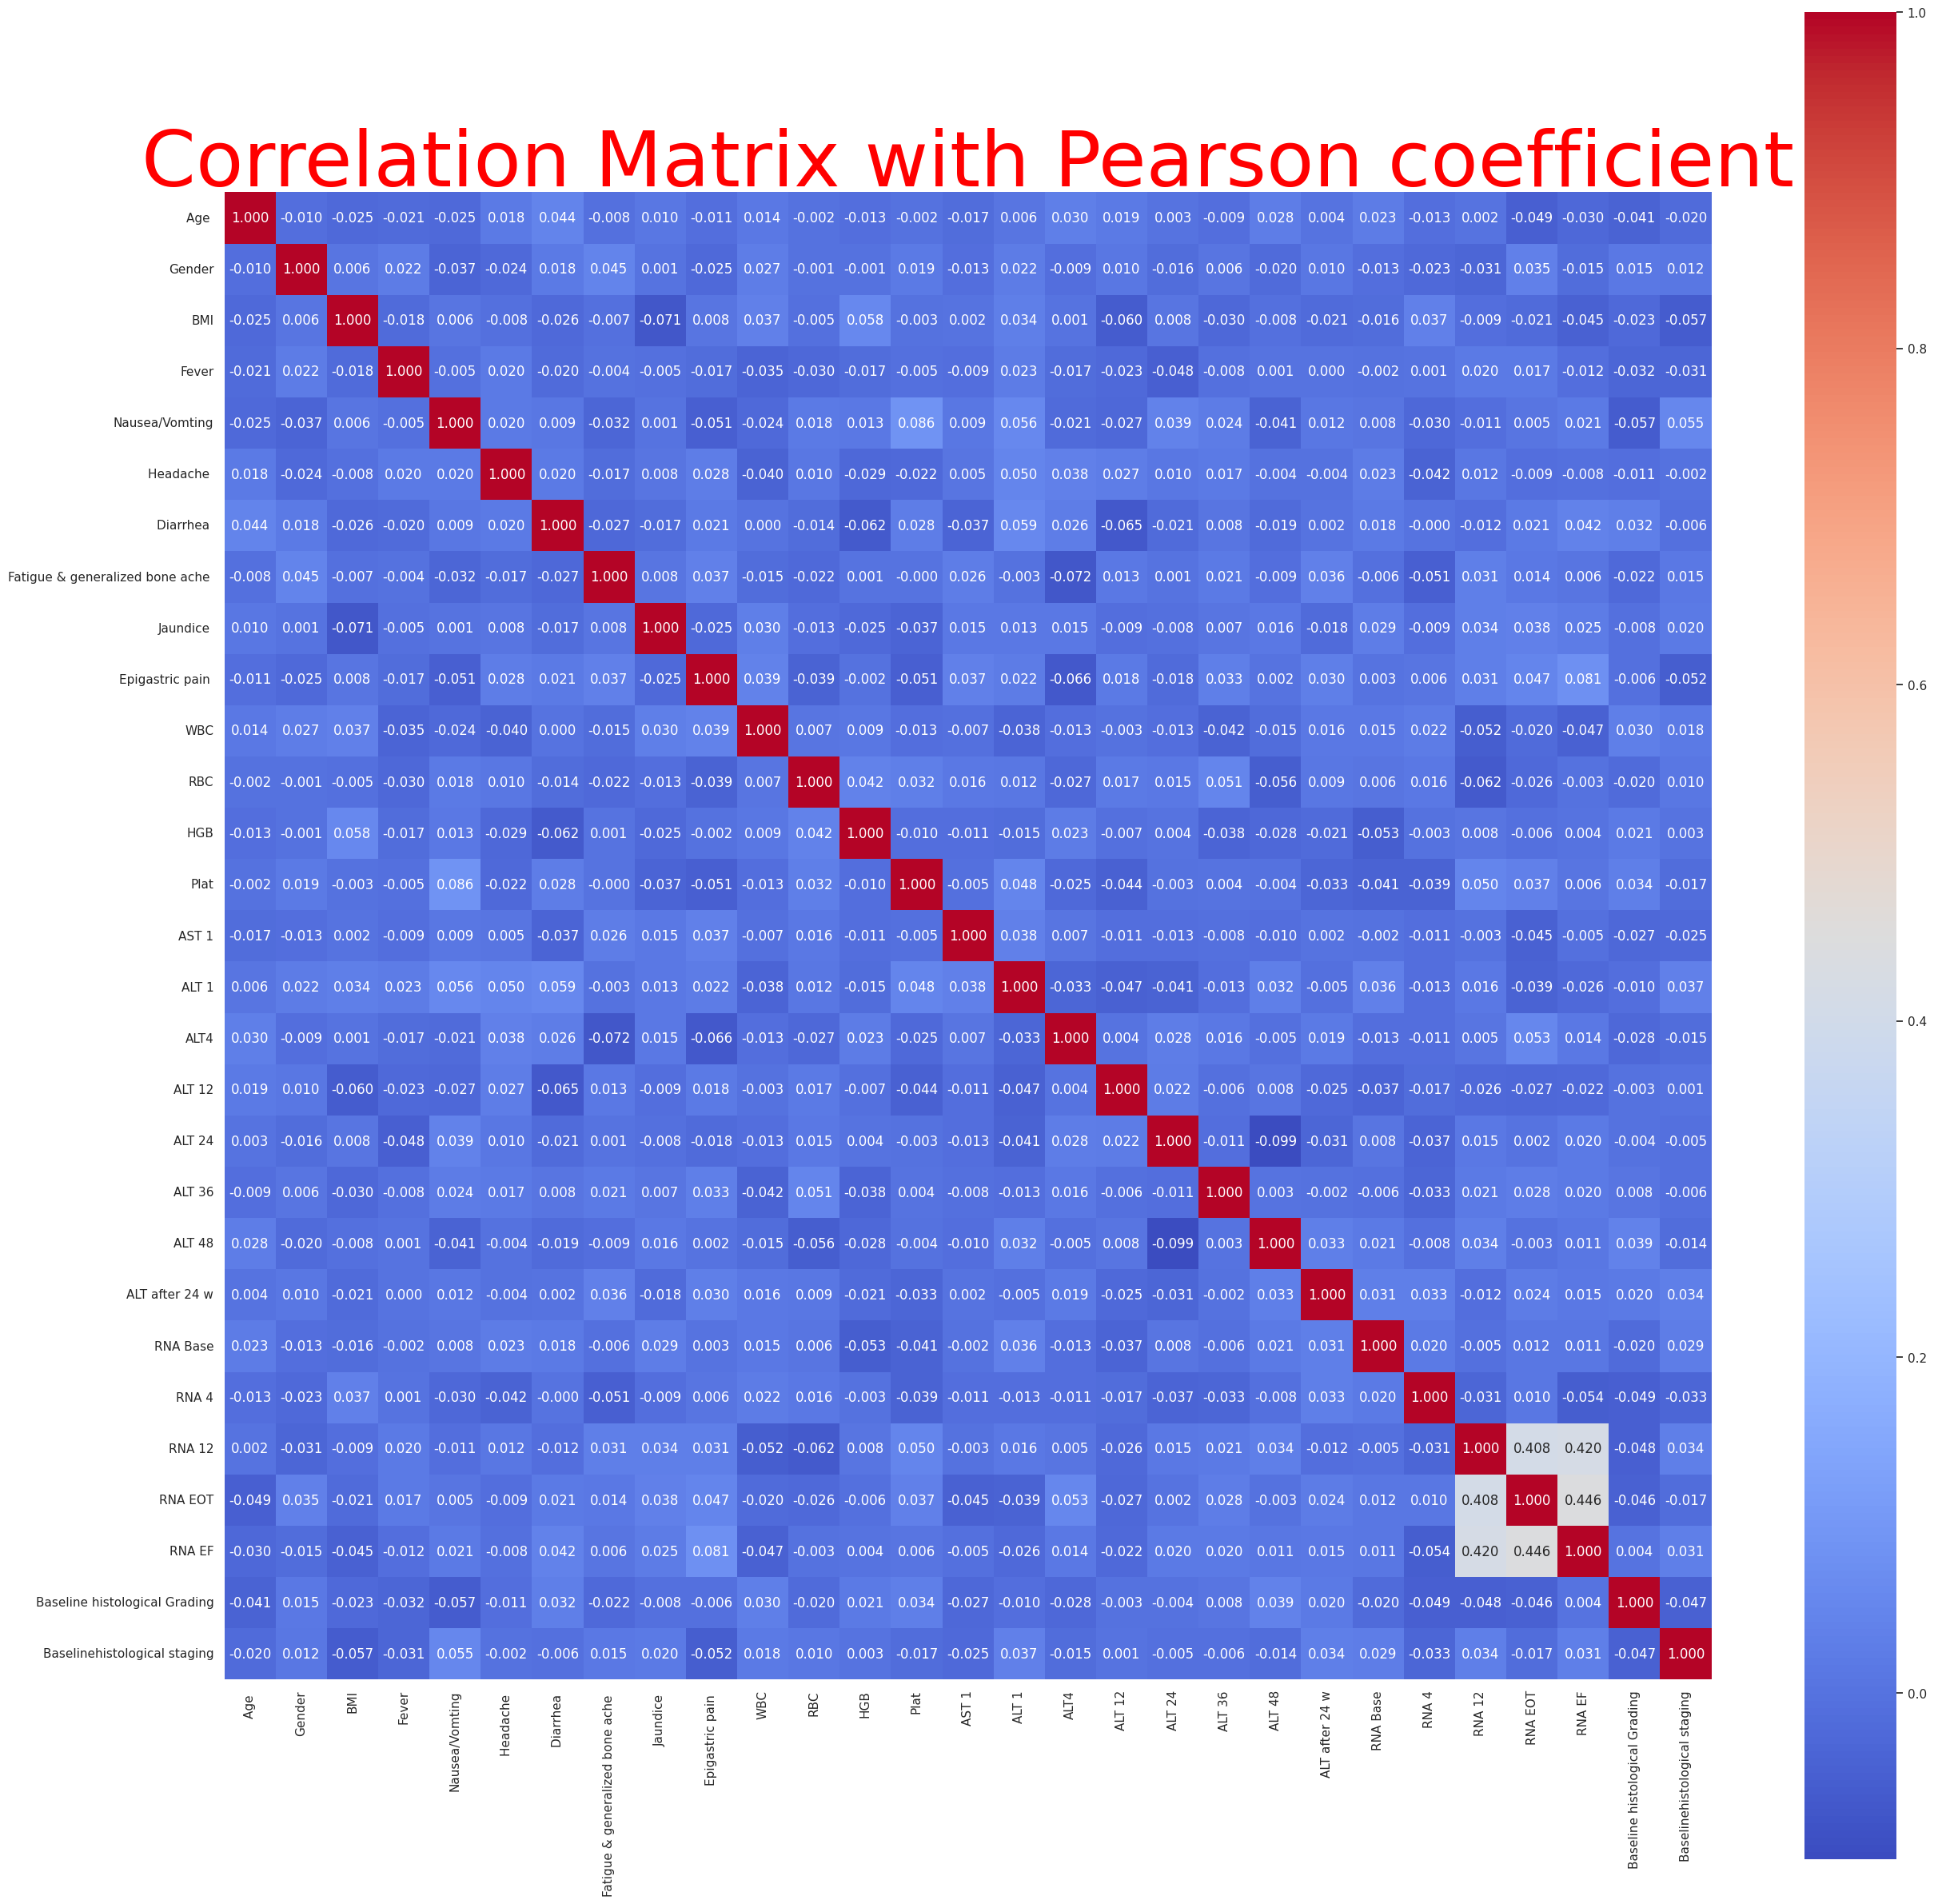
\includegraphics[width=1\textwidth]{corrMatirxPearson.png}
         \caption{Correlazione secondo Pearson}
         \label{fig:PeraonMatrix}
	\end{figure}

    
    \begin{figure}[htbp]
        \centering
		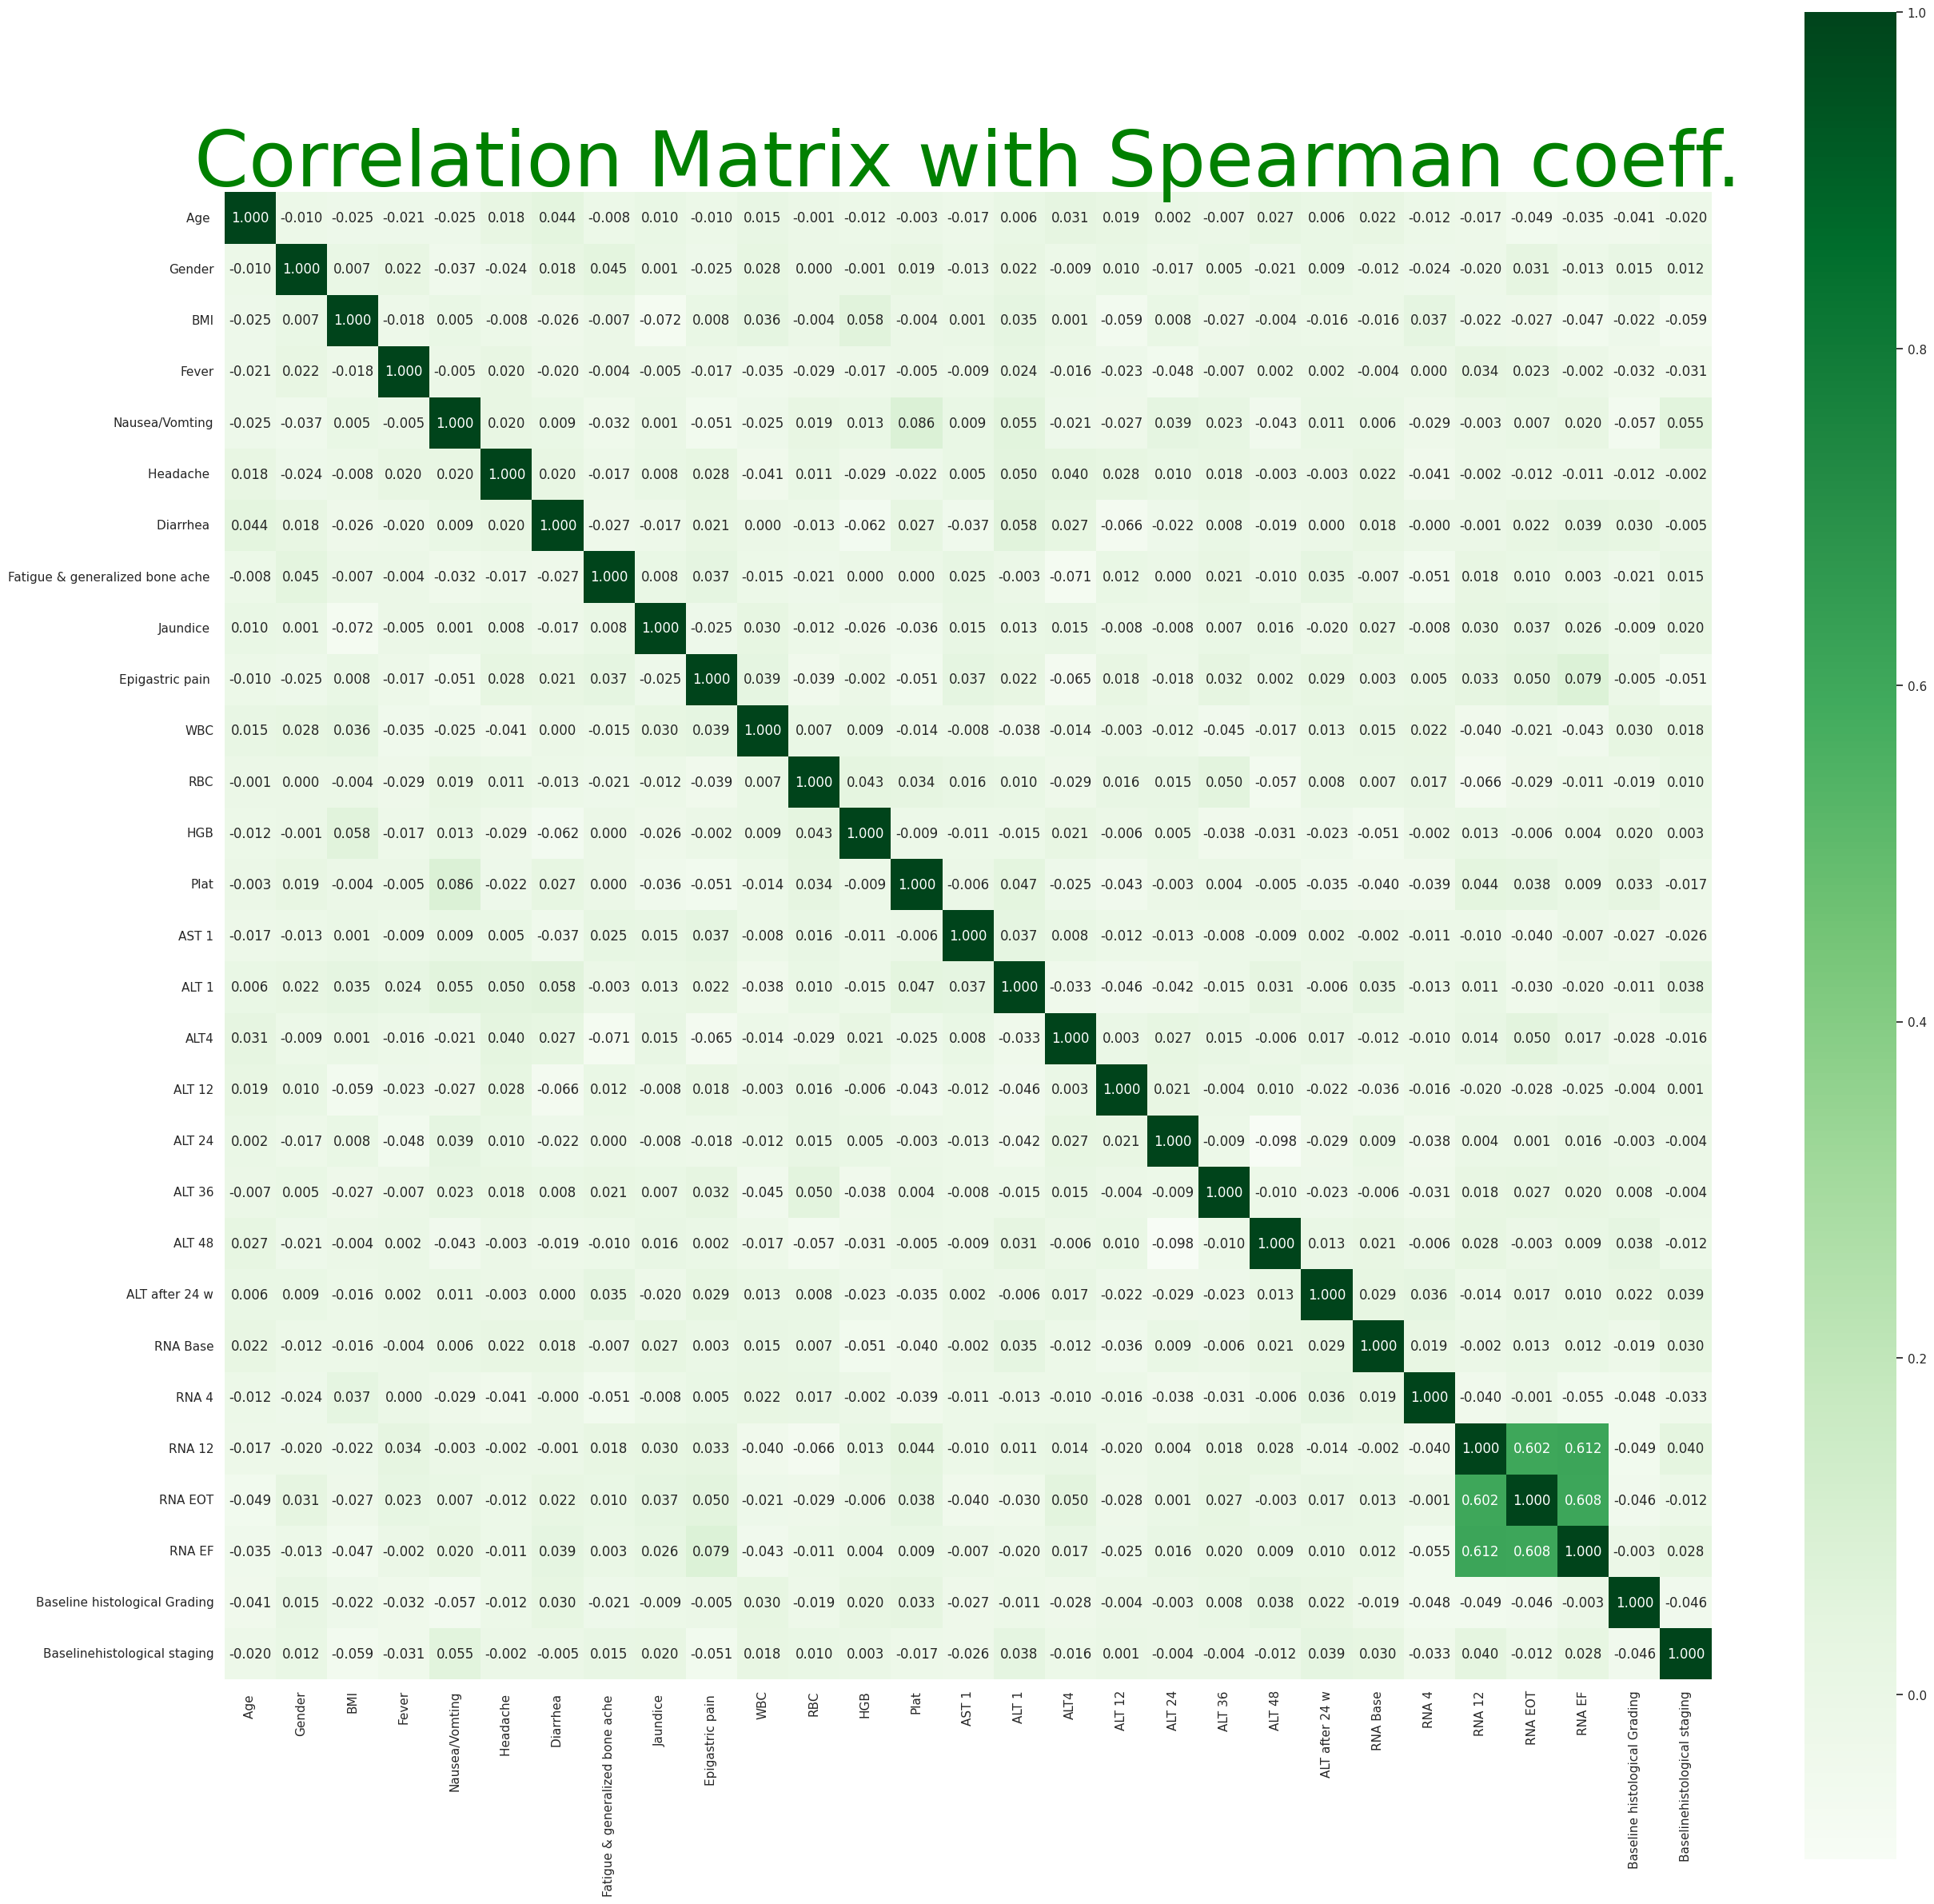
\includegraphics[width=1\textwidth]{corrMatrixSpear2.png}
         \caption{Correlazione secondo Spearman}
        \label{fig:SpearmanMatrix}
	\end{figure}

    
    \begin{figure}[htbp]
        \centering
		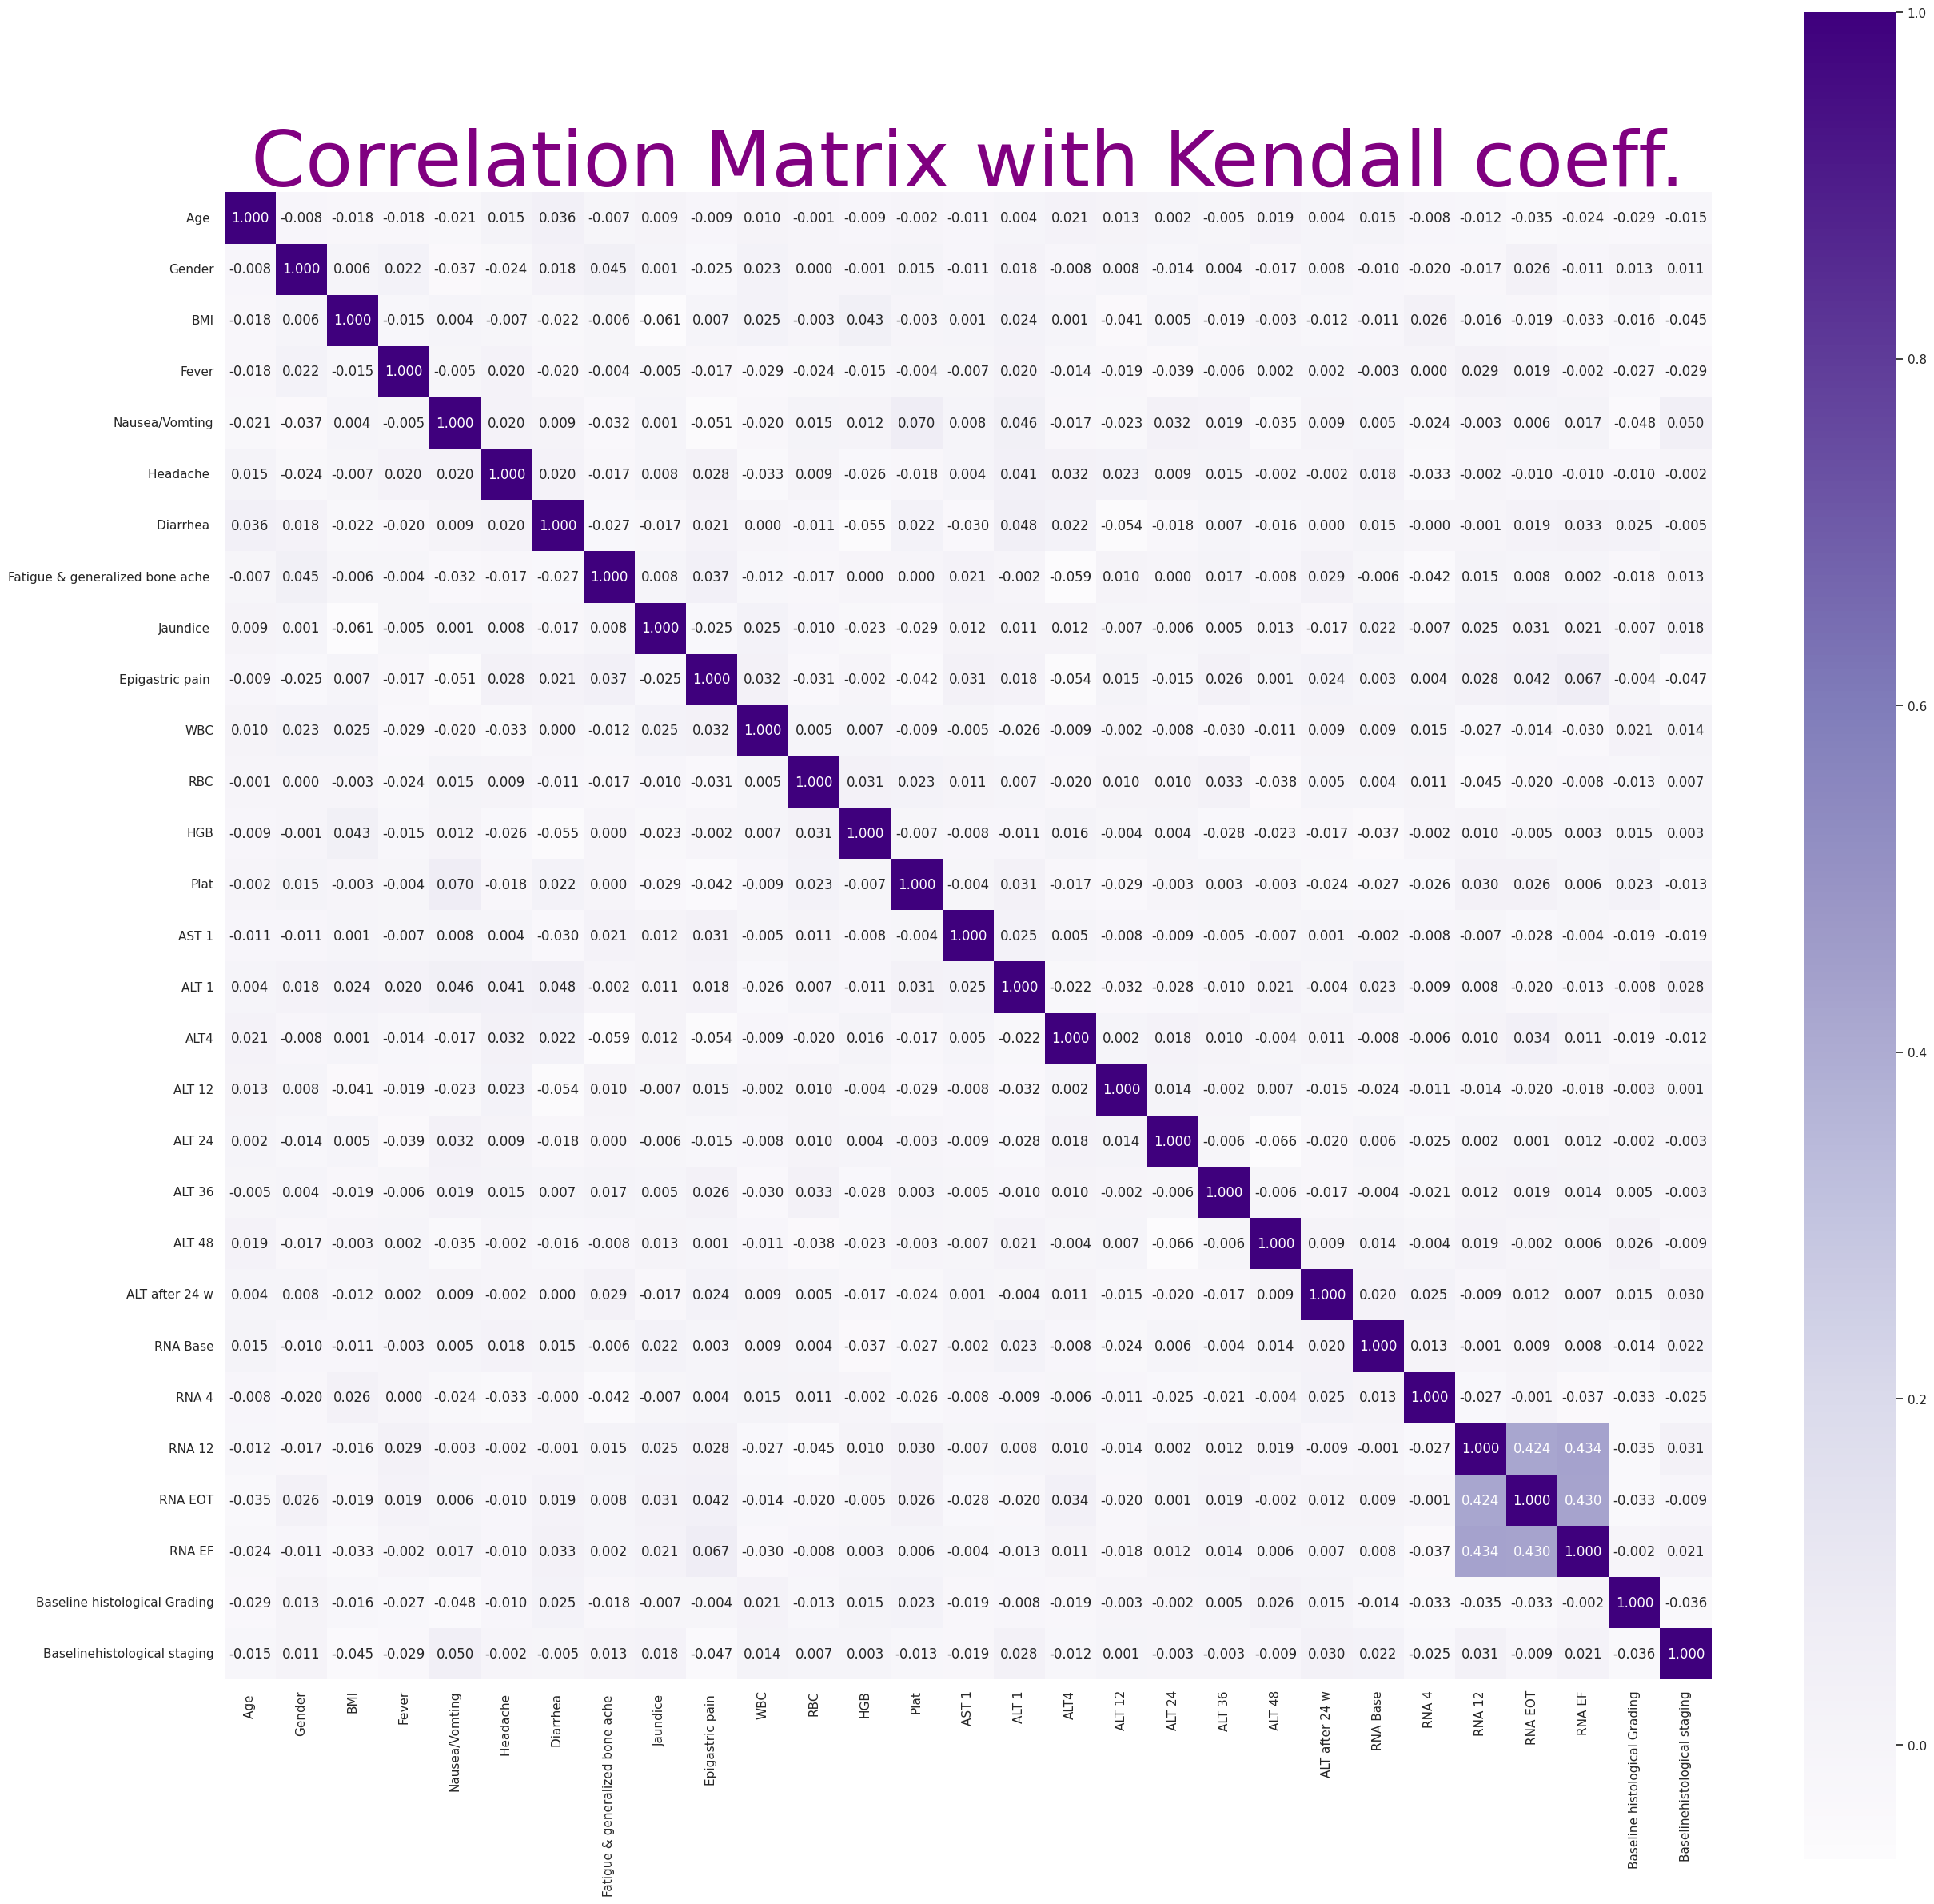
\includegraphics[width=1\textwidth]{corrMatrixKen3.png}
        \caption{Correlazioone secondo Kendall}
        \label{fig:KendallMatrix}
	\end{figure}

    lo studio non ha escluso l'ipotesi di altre tipologie di correlazione le quali non sono state indigate in quanto si è preferito andare avati nell'analisi dei dati per poi cercare di capire come procedere con le future investigazioni.
    
    \vspace{25pt}
	
	
	\subsection{Verifica della qualità dei dati}
    La qualità dei dati è stata analizzata secondo le rigorose regole per tcertificare la validità del dato, questo passo ha visto l'analisi dei valori nulli presenti nel dataset i quali erano assenti e l'analisi di possibili errori di raccolta dei daati nonché della raccolta di outlier. Queste anormalità sono state documentate per poi essere trattate nella fase di preparazione dei dati. Durante questa fase è risultato particolarmente osciso ritrovare le informaziooni a corredo dei dati utilizzati quali la tipologia di test utilizzato per l'attività del HCV, quali metodologie di test del sangue sono state effettuate per calcolare i valori di transaminasi e notevoli problemi che non sono stati risolti si sono incontrati sulla qualità del Baselinehistological grading la scala di mal funzionamento epatica della quale si p capito il range, ma non si è riuscito a interpretare i valori a cosa corrispondano.

    \section{Data preparation}

    \subsection{Data cleaning}
    La pulitura dei dati del nostro dataset ha preso in considerazione più ipotesi in base alla documentazione dei dati raccolti. La prima è stata quella di valutare i valori bassi sui test di ALT ovvero quelòli aventi valore pari a 5.0 come errori di trascrizione del dato e per questo sono stati sostituiti attraverso l'uso di un SimpleImputer con le medie rispettive alle colonne di appatenenza. Per quanto riguarda i valori di RNA dove si è  riscontrato lo stesso problema questi sono stati sostituiti con il minimo valore possibile identificato dal test di Abott ovvero valore pari a 12 unità. Dopo questa fase di pulitura i risultati sono stati salvati per avere un nuovo dataset con queste modifiche e si sono effettuate copie in formato csv e excel. La seconda ipotesi avanzata e che fossero stati errori o outlier e per tali ragioni si sono sostituiti sempre usando il SimpleImputer con la media rispettiva delle colonne di appartenenza e si è ripetuto il processo di creazione di un nuovo data set con conseguente creazione dei file nei formati csv e excel. Infine l'ultima ipotesi avanzata è stata quella che ha visto il valore 5.0 essere stato usato come un valore di default per segnalare la mancanza del valore e poichè sappiamo che è possibile utilizzare modelli resistenti ai valori nulli abbiamo sostituito tali valori con i valori nulli e ripetuto le operazxioni di salvataggio. Per quanto riguarda i dati non chiaramente documentati è stata scelta la politica di scarto  di tale dato e questa politica ha portato a scartare sia la feature "Baselinehistological grading" che la feature "RNA EF" per mancanza di documentazione chiara. 
    
    \subsection{Data construction}
    In questa fase si sono valutate le possibilità di andare a ridurre le dimensione del dataset iniziale che annoverava 29 attributi per limitare la complessità del modello che in seguito avremmo addestrato. Si è pensato quindi di ricorrere alla Principal Component Analysis e di accorpare assieme delle feature che avessere correlazione evidenziata dallo studio delle dipendenze lineari e correlazioni a llivello di dominio per semantica e utilizzo. Seguendo questa idea è stato applicato un processo di data reduction tramite PCA che ha accorpato i valori di AST1 e le osservazioni ripetutte nel tempo di ALT in un unica feature ingegnerizzata che rappresentasse l'andamento deelle transaminasi nel tempo e un'altro accorpamento di dati è stato eseguito sui valori dei test di RNA i quali mostravano una correlazione e hanno creato la nuova feature ingegnerizzata dell'attività polimerasica del HCV durante il trattamento. Questo processo ha permesso di ottenere un nuovo dataset ridotto di dimensioni il quale è stato usato per effettuare un analisi comparativa sull'addestramento di modello con il dataset solomente pulito e quelli addestrati sul dataset pulito e ridotto.

    \subsection{Integrazione e Formatazzione}
    Non è stato necessario integrare il dataset iniziale con ulteriori dati provenienti da forme differenti e raccolti con una metodologia diversa. Per quanto riguarda la formattazione invece sono state apportate leggere modifiche per avere omogeneità dei dati raprresentati come integer a 64 bit e per le feature categoriche si è effettuato una cambiamento di valori in modo da averli in forma booleana 1 e 0.

    \section{Modelling}
    \subsection{Selezione delle tecniche di modellazione}
    La selezione delle tecniche di modellazione ha prodotto un report dettagliato riguardate i modelli utilizzati, le motivazioni indotte ad utilizzare tali modelli e cosa ci ha spiento ad effettuare un'analisi comparativa tra  più modelli. I modelli selezionati appartengono a differenti categorie di modelli utilizzate in base al loro funzionamento e alle ipotesi che essi assumuno di seguito riportiamo i modelli utilizzati:
    
    \begin{itemize}
		\item \textbf{Decision Tree C4.5}
		\item \textbf{GaussianNB}
        \item \textbf{MultinomialNB}
        \item \textbf{BernoulliNB}
        \item \textbf{ComplementNB}
        \item \textbf{Logistic Regression}
        \item \textbf{Ridge Regrtession}
        \item \textbf{SVM coefficiente C}
        \item \textbf{SVM coefficiente Nu}
        \item \textbf{Sthocastic Gradient Descent}
        \item \textbf{Random Forest}
        \item \textbf{Extra Tree}
        \item \textbf{Ada Boost}
        \item \textbf{XGBoost}
        \item \textbf{Gradient Boosting}
        \item \textbf{Perceptron}
        \item \textbf{Multi-layer Perceptron}
	\end{itemize}


	\subsection{Decision Tree C4.5}
    Modello di classificazione che prende in input una collezione di esempi di training $S$ e l'iniseme delle classi $C = \{c_1, c_2, \dots, c_k\}$, ad ogni nodo dell'albero, C4.5 sceglie l'attributo dei dati che più efficacemente suddivide $S$ insieme di campioni in sottoinsiemi in base alle classi. Il criterio di suddivisione è \textit{l'information gain} (differenza di entropia). L'attributo con il più alto guadagno di informazioni normalizzate viene scelto per prendere la decisione. \\
	\textit{l'information gain} per l'attributo di test $t$ sarà:
	
	$$IG(S, t) = E(S) - \sum_i \frac{|S_i|}{|S|}E(S_i)$$ dove $$E(S) = -\sum_{i = 1, \dots, k} Count(c_i, S)\cdot\log(Count(c_i, S))$$

    \subsection{Baysian framework models} 
	Il naive bayes è uno dei modelli del framework bayesiano, si basa sul teorema di Bayes:
	$$P(h|D) = \frac{P(D|h)\cdot P(h)}{P(D)}$$
	Più nello specifico il naive Bayes, considerando ogni instanza del dataset come una tupla di valori $<a_1, a_2, \dots, a_n>$ e l'attributo target che prende i valori da un insieme $V$, va a stimare $P(v_j)$, cioè la probabilità a priori che l'attributo target abbia valore $v_j$, con la frequenza relativa del valore $v_j$ nel dataset $$P(v_j) = \frac{\#istanze\_con\_val\_v_j}{\#istanze\_tot}$$ similmente andrà a stimare la probabilità condizionata $P(a_i|v_j)$ contando quante occorrenze classificate con $v_j$ hanno il valore $a_i$. \\
	Andando ad assumere l'indipendenza condizionale dei valori degli attributi, avremo:
	$$V_{NB} = \max_{v_j \in V}(P(v_j)\prod_{i = 1}^{n} P(a_i|v_j))$$
	Quindi all'istanza $x$ verrà assegnata la classe $v_j$ che ha massimizzato il valore sopra citato.
    \\
    \vspace{25pt}
    
    Il classificatore Gaussian Naive Bayes è particolarmente utile per la classificazione di dati categorici e numerici. In particolare, è in grado di gestire grandi quantità di dati e di lavorare con dati mancanti. Il classificatore Gaussian Naive Bayes utilizza una distribuzione gaussiana per stimare la probabilità di appartenenza di un'osservazione ad una classe. In altre parole, il classificatore calcola la probabilità che un'osservazione appartenga ad una classe specifica utilizzando la distribuzione gaussiana delle caratteristiche di quella classe. La sua ipotesi di partenza e che i dati si distribuiscano come una gaussiana.
    \\
    \vspace{25pt}

    
    Il classificatore Multinomial Naive Bayes è un algoritmo di apprendimento automatico utilizzato per la classificazione di dati. Il classificatore Multinomial Naive Bayes è particolarmente utile quando si hanno a disposizione dataset di grandi dimensioni e con molte categorie, in quanto è in grado di gestire un grande numero di categorie senza compromettere le prestazioni. Questo classificatore  può essere utilizzato anche in presenza di dati mancanti o rumorosi.
    \\
    \vspace{25pt}

     
    Il classificatore di BernoulliNB assume che i dati siano distribuiti secondo distribuzioni di Bernoulli multivariate, per cui possono esserci più caratteristiche, ma si presume che ciascuna di esse sia una variabile a valore binario (Bernoulli, booleano). Pertanto, questa classe richiede che i campioni siano rappresentati come vettori di caratteristiche a valori binari; se viene consegnato qualsiasi altro tipo di dati, un'istanza BernoulliNB può binarizzare il suo input (a seconda del binarizeparametro).
    \\
    \vspace{25pt}

    
    Il classificatore ComplementNB è una variante del classificatore Naive Bayes che è stato progettato per affrontare il problema della classificazione multiclasse sbilanciata.Il CNB è particolarmente utile quando si lavora con dataset in cui le classi non sono bilanciate, ovvero quando alcune classi hanno molte più istanze rispetto ad altre. In questi casi, il classificatore Naive Bayes standard può avere problemi a classificare correttamente le classi minoritarie. Il CNB risolve questo problema introducendo un termine di complemento nella stima delle probabilità delle classi.In pratica, il CNB funziona calcolando la probabilità di appartenenza di un'istanza a ciascuna classe, utilizzando la regola di Bayes. La classe con la probabilità più alta viene quindi assegnata all'istanza. Tuttavia, a differenza del classificatore Naive Bayes standard, il CNB utilizza un termine di complemento nella stima delle probabilità delle classi. Questo termine di complemento è calcolato come la somma delle frequenze delle feature per tutte le classi tranne quella corrente, diviso per la somma delle frequenze totali delle feature.
    \\
    \vspace{25pt}
    \subsection{Regression based models}
    I modelli di classificazione basati su regressione sono un tipo di approccio utilizzato per risolvere problemi di classificazione utilizzando algoritmi di regressione. Invece di assegnare una classe direttamente ai dati di input, questi modelli stimano una variabile continua che rappresenta la probabilità di appartenenza a una determinata classe.
    \\
    \vspace{25pt}

     La regressione logistica è un modello di classificazione utilizzato per prevedere la probabilità di appartenenza di un'osservazione a una delle classi target. Questo modello utilizza una funzione logistica per calcolare la probabilità di appartenenza a una classe. La funzione logistica è una funzione sigmoide che restituisce un valore compreso tra 0 e 1. Questo valore rappresenta la probabilità che l'osservazione appartenga alla classe positiva. Durante la fase di addestramento, il modello di regressione logistica utilizza un insieme di dati di addestramento per stimare i coefficienti del modello. Questi coefficienti vengono utilizzati per calcolare la probabilità di appartenenza a una classe per ogni osservazione. Durante la fase di classificazione, il modello di regressione logistica utilizza la probabilità calcolata per assegnare un'osservazione a una delle due classi possibili. In genere, viene utilizzato un valore di soglia per determinare la classe finale. Se la probabilità calcolata supera la soglia, l'osservazione viene assegnata alla classe positiva, altrimenti viene assegnata alla classe negativa.
     \\
     \vspace{25pt}


     La regressione ridge è un modello di regressione lineare che utilizza una tecnica di regolarizzazione chiamata "ridge penalty" per ridurre la varianza del modello e prevenire l'overfitting. La regressione ridge è spesso utilizzata per problemi di regressione in cui il numero di variabili predittive è maggiore del numero di osservazioni. Il modello di regressione ridge è simile alla regressione lineare, ma include un termine di regolarizzazione nella funzione di costo. Questo termine di regolarizzazione è proporzionale al quadrato della norma L2 dei coefficienti del modello, che significa che i coefficienti del modello vengono penalizzati se diventano troppo grandi. Questo aiuta a ridurre la varianza del modello e a prevenire l'overfitting. Il parametro di regolarizzazione, chiamato "lambda", controlla l'importanza della penalizzazione. Un valore di lambda più alto aumenta la penalizzazione e riduce la complessità del modello, mentre un valore di lambda più basso riduce la penalizzazione e aumenta la complessità del modello.

    \subsection{Support Vector Machine models}
    I modelli di classificazione basati su Support Vector Machine (SVM) sono algoritmi di apprendimento automatico che utilizzano un approccio di apprendimento supervisionato per la classificazione dei dati. L'obiettivo principale di un modello SVM è quello di trovare un iperpiano che separi i dati in due classi.
    \\
    \vspace{25pt}

    Il modello di classificazione Linear SVM (Support Vector Machine) è un algoritmo di apprendimento automatico che viene utilizzato per la classificazione. L'obiettivo del modello è quello di trovare un iperpiano che separi i dati, tale iperpiano viene definito come una combinazione lineare delle variabili predittive, dove ogni variabile ha un peso associato. L'obiettivo dell'algoritmo è quello di trovare i pesi ottimali che massimizzano la distanza tra l'iperpiano e i punti più vicini delle due classi, chiamati vettori di supporto. Il modello di classificazione Linear SVM è particolarmente utile quando i dati sono linearmente separabili, ovvero quando esiste un iperpiano che separa perfettamente le due classi.
    \\ 
    \vspace{25pt}

    Il modello di classificazione NU Support Vector Machine (SVM) è un algoritmo di apprendimento automatico per la classificazione binaria e multiclasse. Il parametro NU controlla il numero di support vector e la larghezza della regione di decisione. In altre parole, NU controlla la complessità del modello e la sua capacità di generalizzazione. Un valore di NU più basso indica un modello più complesso, mentre un valore di NU più alto indica un modello più semplice. Il modello di classificazione NU SVM utilizza una funzione kernel per mappare i dati di input in uno spazio di dimensioni superiori, dove è più facile separare le classi. La funzione kernel più comune utilizzata con il modello NU SVM è la funzione RBF (Radial Basis Function).
    \\
    \vspace{25pt}

    Il modello di classificazione basato su SVM (Support Vector Machine) con coefficiente C è un algoritmo di apprendimento automatico supervisionato utilizzato per la classificazione di dati. Il parametro C è un parametro di regolarizzazione che controlla la penalizzazione degli errori di classificazione. Un valore elevato di C indica una penalizzazione elevata degli errori di classificazione, il che significa che il modello cercherà di classificare correttamente tutti i punti di addestramento, anche se questo significa creare un iperpiano più complesso. Al contrario, un valore basso di C indica una penalizzazione bassa degli errori di classificazione, il che significa che il modello cercherà di creare un iperpiano più semplice, anche se questo significa classificare alcuni punti di addestramento in modo errato. Il modello di classificazione basato su SVM con coefficiente C è in grado di gestire dati non lineari utilizzando una tecnica chiamata "kernel trick". Questa tecnica consiste nell'applicare una funzione di trasformazione ai dati di addestramento per proiettarli in uno spazio di dimensioni superiori, dove è più facile trovare un iperpiano che separi le classi. 
    \\
    \vspace{25pt}
   
    \subsection{Ensemble learning models}
    I modelli di ensemble machine learning sono un insieme di modelli di machine learning che lavorano insieme per migliorare le prestazioni complessive del modello. Questi modelli combinano le previsioni di più modelli di machine learning per ottenere una previsione finale più accurata rispetto a quella di un singolo modello.La loro forza sta nel supporto che ottengono dal gruppo di modelli che viene ad essere addestrato. L'idea generale dietro a questo tipo di apprendimento di macchina è che se ho più modelli addestrati dove uno commetterà degli errori tali errori saranno coperti o riparati dagli altri modelli, questo perché la decisione finale è una aggregazione dei risultati di ogni modello.
    \\
    \vspace{25pt}

    \subsubsection{Bootstrap Aggregating}
    Il Bagging abbreviazione che sta per il processo di Boostrap Aggregatin utilizza più modelli di machine learning addestrati su campioni di dati diversi per ridurre la varianza e migliorare la precisione delle previsioni. Ogni singolo classificatore di addestra su una porzione casuale di dati, questo riesce a limitare l’overfitting e aumentare le sue capacità predittive. In questa aggregazione di modelli, viene utilizzata una tecnica chiamata boostrap: alcuni dati possono comparire contemporaneamente in più modelli mentre altri potrebbero non comparire mai. Questa tecnica si chiama anche campionamento causale con rimpiazzo. I seguenti rappresentano i modelli di ensemble basati su Bagging che abbiamo utilizzato durante il progetto.
    \\
    \vspace{25pt}

    \begin{itemize}
		\item \textbf{Random Forest}
		\item \textbf{Extra Tree}
    \end{itemize}

    \vspace{25pt}

    
    Un classificatore Random Forest è un algoritmo di apprendimento automatico che utilizza un insieme di alberi decisionali per effettuare la classificazione di dati. È un tipo di algoritmo di apprendimento ensemble, in cui diversi modelli vengono combinati per ottenere una previsione più accurata. Il processo di creazione di un classificatore Random Forest inizia con la creazione di un insieme di alberi decisionali. Ogni albero viene addestrato su un sottoinsieme casuale dei dati di addestramento e utilizza una tecnica chiamata "bagging" per selezionare casualmente le caratteristiche da utilizzare durante la creazione del modello. Questo aiuta a ridurre la varianza e il rischio di overfitting. Durante la fase di classificazione, ogni albero nel Random Forest emette una previsione e la classe finale viene determinata tramite votazione maggioritaria. In altre parole, la classe che ottiene il maggior numero di voti tra gli alberi viene selezionata come previsione finale. I classificatori Random Forest sono noti per la loro capacità di gestire grandi quantità di dati e di variabili predittive. Sono anche in grado di gestire dati mancanti e di gestire variabili categoriche senza la necessità di codificarle in modo esplicito.
    \\
    \vspace{25pt}

    Un modello di classificazione Extra Trees dove extra sta per "Estremamente Randomizzato". Questo è un algoritmo di apprendimento automatico con supervisione che utilizza un insieme di alberi decisionali per effettuare la classificazione di dati. È simile al modello Random Forest, ma con alcune differenze chiave nella selezione delle caratteristiche e nella creazione degli alberi.In un modello Extra Trees, le caratteristiche vengono selezionate casualmente per ogni albero decisionale, a differenza del modello Random Forest in cui le caratteristiche vengono selezionate utilizzando un criterio di massima importanza. Inoltre, durante la creazione degli alberi, i punti di separazione vengono scelti casualmente, a differenza del modello Random Forest in cui vengono utilizzati criteri di separazione più sofisticati. L'utilizzo di una selezione casuale delle caratteristiche e dei punti di separazione aiuta a ridurre la varianza e il rischio di overfitting, ma può anche aumentare la bias. Tuttavia, questo trade-off può essere gestito regolando i parametri del modello.
    \\
    \vspace{25pt}


    \subsubsection{Boosting}
    Utilizza più modelli di machine learning addestrati sequenzialmente per migliorare la precisione delle previsioni. Ogni modello successivo si concentra sui campioni di dati che sono stati classificati in modo errato dal modello precedente. Nel boosting quindi ogni modello viene costruito in modo sequenziale in base agli errori del modello precedente. Nel processo di apprendimento i dati vengono forniti al primo classificatore, il quale effettua una prediction. Nel classificatore successivo che verrà ad essere addestrato viene dato più peso alle istanze classificate in modo sbagliate dal precedente classificatore. In questo modo l’enfasi viene posta sugli errori dei classificatori precedenti. I seguenti modelli di ensemble basati su boosting sono quelli utilizzati nel progetto:
    \\
    \vspace{25pt}

     \begin{itemize}
		\item \textbf{Ada Boost}
		\item \textbf{XgBoost}
        \item  \textbf{Gradient Boosting}
    \end{itemize}

     \vspace{25pt}

     AdaBoost o anche conosciuto come Adaptive Boosting è un algoritmo di apprendimento automatico supervisionato di tipo ensemble learning che combina diversi modelli di apprendimento automatico deboli per creare un modello di apprendimento automatico forte. L'idea alla base di AdaBoost è quella di addestrare una serie di modelli deboli, ciascuno dei quali ha una precisione leggermente superiore al caso casuale, e poi combinare questi modelli deboli in modo da creare un modello forte. Il processo di addestramento di AdaBoost inizia con l'addestramento di un modello di apprendimento automatico debole sul set di dati di addestramento. Successivamente, viene calcolato l'errore di classificazione del modello debolmente addestrato e viene assegnato un peso maggiore agli esempi di addestramento che sono stati classificati erroneamente. In questo modo, i modelli successivi si concentrano sui dati che sono stati classificati erroneamente dai modelli precedenti. Durante il processo di addestramento, ogni modello debole viene assegnato un peso in base alla sua precisione. I modelli più precisi ricevono un peso maggiore, mentre i modelli meno precisi ricevono un peso minore. In questo modo, i modelli più precisi hanno un maggiore impatto sulla previsione finale. Durante la fase di classificazione, ogni modello debole emette una previsione e la classe finale viene determinata tramite votazione pesata
    \\
    \vspace{25pt}

    XGBoost anche conosciuto come eXtreme Gradient Boosting è un algoritmo di apprendimento automatico supervisionato basato su alberi decisionali che utilizza un approccio di boosting per creare un modello di classificazione. È stato sviluppato per migliorare le prestazioni degli algoritmi di gradient boosting standard. Il modello XGBoost utilizza una combinazione di alberi decisionali deboli, che sono alberi decisionali con una profondità limitata e una capacità di generalizzazione limitata. Questi alberi decisionali deboli vengono addestrati in sequenza, in modo che ogni nuovo albero aggiunto si concentri sui campioni che sono stati classificati in modo errato dai modelli precedenti. In questo modo, il modello XGBoost cerca di migliorare continuamente la sua capacità di classificazione. Durante la fase di addestramento, XGBoost utilizza una funzione di perdita personalizzata per valutare la qualità delle previsioni del modello. Questa funzione di perdita tiene conto della complessità del modello e della precisione delle previsioni, in modo da trovare il giusto equilibrio tra la complessità del modello e la sua capacità di generalizzazione. Inoltre, XGBoost utilizza una tecnica chiamata "pruning" per rimuovere i rami dell'albero decisionale che non contribuiscono significativamente alla capacità di classificazione del modello. Questo aiuta a ridurre la complessità del modello e a migliorare le sue prestazioni.
    \\
    \vspace{25pt}

    Il modello di classificazione Gradient Descent Boosting (GDB) è un algoritmo di apprendimento automatico che utilizza una combinazione di alberi decisionali per effettuare la classificazione dei dati. È un tipo di algoritmo di apprendimento ensemble, in cui diversi modelli vengono combinati per ottenere una previsione più accurata. Il processo di creazione di un modello GDB inizia con la creazione di un albero decisionale. Questo albero viene addestrato sui dati di addestramento e utilizza una tecnica chiamata "boosting" per selezionare le caratteristiche più importanti da utilizzare durante la creazione del modello. In particolare, il boosting assegna un peso maggiore ai dati che sono stati classificati in modo errato dal modello precedente, in modo da concentrarsi sui dati più difficili da classificare. Durante la fase di classificazione, ogni albero nel modello GDB emette una previsione e la classe finale viene determinata tramite votazione maggioritaria. Tuttavia, a differenza di altri algoritmi di apprendimento ensemble, come il Random Forest, il modello GDB utilizza una tecnica chiamata "gradient descent" per ottimizzare la combinazione degli alberi decisionali.
    \\
    \vspace{25pt}
    
    \subsection{Perceptron based models}
    Il modello Perceptron Classifier è un tipo di algoritmo di apprendimento automatico utilizzato per la classificazione. Questo modello è composto da uno o più input, pesi associati a ciascun input e una funzione di attivazione. Gli input rappresentano le caratteristiche o attributi dei dati di input, mentre i pesi determinano l'importanza relativa di ciascun input nel processo decisionale del perceptron. La funzione di attivazione decide se il perceptron deve essere attivato o meno sulla base del risultato della combinazione lineare degli input e dei pesi. L'addestramento del modello Perceptron Classifier coinvolge il processo di aggiornamento dei pesi in modo da ridurre l'errore tra l'output previsto e l'output desiderato. Durante l'addestramento, i dati di addestramento vengono presentati al perceptron, e per ciascuna istanza, il perceptron calcola l'output previsto in base ai pesi correnti e alla funzione di attivazione. Se l'output previsto è corretto, i pesi rimangono invariati. In caso contrario, i pesi vengono aggiornati per ridurre l'errore. L'algoritmo Perceptron Classifier può essere iterato fino a quando i pesi convergono a un valore stabile o fino a quando viene raggiunto un numero massimo di iterazioni predefinite. Una volta che il modello è addestrato, può essere utilizzato per effettuare previsioni su nuovi dati di input assegnando loro una classe o un'etichetta sulla base delle caratteristiche rilevanti apprese durante l'addestramento.
    
    Il MLP (Multilayer Perceptron) Classifier è un tipo di modello di classificazione utilizzato nell'apprendimento automatico. Si basa sul concetto di reti neurali artificiali, che sono ispirate al funzionamento dei neuroni biologici nel cervello umano. Questo modello è costituito da un insieme di strati o "livelli" di neuroni artificiali chiamati neuroni nascosti, che collegano l'input ai risultati di output. Ogni neurone in un livello è collegato a tutti i neuroni nel livello successivo, formando una struttura di rete multi-strato. L'input viene presentato al primo livello di neuroni, chiamato strato di input, e l'output viene generato nel livello finale, chiamato strato di output. Gli strati intermedi, chiamati strati nascosti, contengono neuroni che elaborano e trasmettono informazioni attraverso la rete. Ogni neurone in un MLP Classifier ha pesi associati ai collegamenti tra gli strati. Durante l'addestramento del modello, questi pesi vengono regolati in base all'errore tra l'output previsto e l'output desiderato, utilizzando algoritmi di retropropagazione dell'errore. L'obiettivo è ridurre gradualmente l'errore di classificazione e ottimizzare i pesi in modo che il modello possa fare previsioni accurate su nuovi dati. Per attivare i neuroni in un MLP Classifier, viene utilizzata una funzione di attivazione non lineare. La funzione di attivazione introduce la non linearità nella rete, consentendo al modello di apprendere relazioni complesse tra le caratteristiche di input e le etichette di output. Alcune delle funzioni di attivazione comuni utilizzate in un MLP Classifier sono la funzione sigmoide, la funzione tangente iperbolica (tanh) e la funzione ReLU (Rectified Linear Unit).
    
    Questi due modelli sono stati ambedue implementati avendo visto che le funzioni di regressione per la classificazione come la Logistic regression e la ridge regression avevano dato dei risultati che lasciavano sperare che si potesse migliore. Prima di addestrare questi due modelli sono state fatte ulteriori modificahe al dataset in particolare si è applicato un econder che ha normalizzato tutte le colonne di input tra [0,1] al fine di non creare sbilanciamenti dato la grossa differenza in ordine di grandezza dei numeri trattati per ogni colonna. Dopo aver addestrato ambue due il modelli si sono ottenuti risultati scarsi e anche a seguito di una procedura di semi-ottimizzazione voltqa a trovare una combinazione adeguata di parametri performanti non si sono ottenuti buoni risultati e in particolare non si è riuscito a battere la moda.
    

    \section{Ottimizzazione dei migliori modelli addestrati}
    Il primo modello ad essere stato selezionato per l'ottimizzazione dei parametri è stato il Decision Tree C4.5. Il processo di ottimizzazione ha previsto tramite una funzione basata su grid search l'ottimizzazione indipendente di ogni paramtro del modello per comprendere meglio come il parametro reaggisce a differenti modifiche. Sono stati eseguiti dei plot che vedono l'ottimizzazione del singolo parametro in relazione all'aumento o diminuzione di accurancy. Successivamente tramite un processo di ottimizzazione congiuta è stata utilizzata una beam search per la ricerca nello spazio dei paramtri della più efficiente e performante combinazione di parametri da utilizzare. Infine una volta estratta la combinazione ottimale è stato rieseguito il test di ottimizzazione sul numero dei fold per la cross-validation. Queste ottimizzazione ci hanno permesso di superare il lower bound che ci siamo imposti in partenza ovvero battere l'accuratezza della moda che risultava pari a 26.137\% e il nostro albero ottimizzato a riportato valori di accuratezza superiori al 28\%, ma sfortunatamente acora troppo bassi per una reale implementazione del modello nella sanità.
    \\

    L'ottimizzazione è stata estesa anche ai 2 modelli più performanti di Naive Bayes ovvero al ComplementNaive Bayes e al Bernoulli Naive Bayes quest'ultimo si è rivelato incogruente con il task scelto a causa della forzatura di binarizzazione che adopera sulle feature e dopo gli esperimenti condotti esso è risultato equivalente alla moda, l'altro invece ha dato dei buoni risultati capaci in ogni situazione di battere la moda con un accurancy che varia tra 26.2\% e 27.2\%. Infine abbiamo condotto anche alcuni esperimenti di ottimizzazione sul logistic regression classifier il quale dopo ottimizzazione dei parametri è stato anche esso capace di superare la moda. Nonostante le attente e scrupolose ottimizzazioni di questi modelli essi si rivelano tutti estremamente inefficienti per il nostro scopo.
    \\
    \vspace{25pt}

	\section{Conclusioni}
	A fine degli esperimenti condotti sino ad ora non siamo riusciti ancora a raggiungere gli obiettivi di data mining fissati e neppure a soddisfare gli obiettivi di business. Nonostante queeti insuccessi e vista la visione con cui è stato realizzato tale progetto si lasciano ancora porte aperte a future sperimentazioni e nuove ottimizzazioni dei modelli già addestrati con l'obiettivo di riuscire a creare un classificatore che abbiamo almeno il 70\%-80\% di accuratenzza nel predire lo stadio della fibrosi e poter quidndi essere integrato nell'assistenza di questi pazienti a supporto dei medici e della sanità. 
	
\end{document}